\chapter{Problem Statement \& Proposed Solution} \label{chap:proposed-solution}

\section{Problem Statement}

* What?

Current Reinforcement Learning algorithms are not prepared to consider graph topology features of the environent in the decision making process. Additionally, they lack an efficient method for generalizing the learned policies in dynamic topologies that suffer changes over time.

* Why?

Graphs are ubitquotous representations that can serve to instinctively represent several problems and domains. In several problems these representations reveal underlying features that can't be naturally represented by plain euclidean data. However, this problem becomes even more complex considering that graph data is complex and there is a need for designing methods that efficiently extract representations

* Where?

This problem can be observed in several studies where RL models are applied to domains where the intricate relationships between the objects may be relevant for mapping the observable environment states to optimal action policies. Smart Grid services are an example of such domains, given that power grids can be viewed as complex networks of nodes (consumers or producers) and powerlines connecting them that transport energy. More specifically, this dissertation's will

* Who?

This deeply affects the performance of decision-making systems inserted in graph-based domains.

* When?

More and more, this problem attracts the curiosity of academics. With the recent advancements of GNNs the popularity around \ac{GRL} has rose because of their excellent efficiency in creating optimal graph representations and other graph machine learning problems.

* How? 

This problem was observed by conducting a thorough literature review of the relevant works in \ac{GRL} and \ac{RL} solutions for the \ac{DED} problem. It was concluded that plain \ac{RL} approaches were not sufficient for extracting and generalizing (dynamic) graph topology features. The research conducted in \ac{GRL} has shown success in tackling this issue.

\section{Requirements}

\subsection{Functional}

\begin{table}[h!]
	\centering
	\caption{Functional Requirements}
	\begin{tabular}{|P{2cm}|P{4cm}|p{6cm}|  }
		\hline
		\textbf{Requirement} & \textbf{Title} & \textbf{Description} \\
		\hline
		F1 & Optimization & The system should be able to optimize the dispatch of generation resources in real-time to meet the time-varying load demands \\
		\hline
		F2 & Learning Capability & The system must learn from past experiences and optimize its dispatch policies over time \\
		\hline
		F3 & Adaptability & The system should adapt to changes in the power grid topology or in load patterns \\
		\hline
		F4 & Constraints & The system should fullfil the various power grid constraints, namely power balance, generator constraints, ramp rate limits and \ac{ESS} Constraints \\
		\hline
		F5 & Scalability & The system must handle scenarios of different sizes, ranging from small to complex power distribution grids \\
		\hline
	\end{tabular}
\end{table}

\subsection{Non-functional}

\begin{table}[h!]
	\centering
	\caption{Non-functional Requirements}
	\begin{tabular}{|P{2cm}|P{4cm}|p{6cm}|  }
		\hline
		\textbf{Requirement} & \textbf{Title} & \textbf{Description} \\
		\hline
		NF1 & Performance & \\
		\hline
		NF2 & Reliability & \\
		\hline
		NF3 & Usability & \\
		\hline
		NF4 & Security & \\
		\hline
		NF5 & Maintainability & \\
		\hline
		
		\hline
	\end{tabular}
\end{table}

\subsection{Structural}

\section{Architecture}



\section{Methodology}

Concerning the methodology for the research process, the main focus lies on researching the relevant approaches for implementing \ac{GRL} algorithms

\section{Evaluative Methods}

\section{Work Plan}

\begin{figure}
	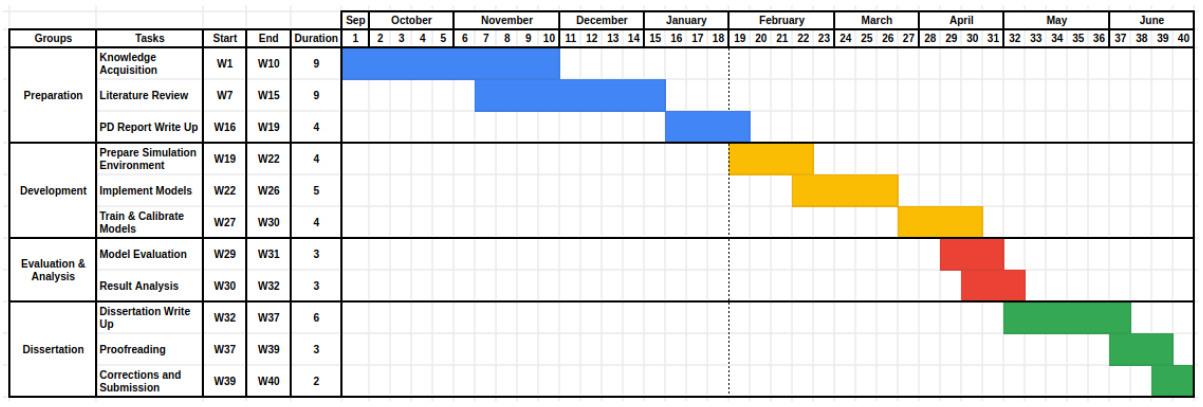
\includegraphics[width=1.0\linewidth]{./figures/gantt-chart.png}
\end{figure}

